%\section{Methodology}\label{sec:methodology}
The research methodology starts in \cref{subsec:algorithm} with a description of the minimum dominating set (MDS) approximation algorithm by Alipour, the SNN implementation of this algorithm by Diehl et al., and the implemented form %TODO: form or forms? 
of brain adaptation \cite{alipour2020distributed}\cite{diehl}. Since the overarching research project aims at performing physical radiation tests, \cref{subsec:hardware} specifies the hardware that is used for testing, and how the radiation effects are simulated. The test procedure is detailed in \cref{subsec:testing}.

\subsection{Algorithm Selection}\label{subsec:algorithm}
The MDS approximation as presented by Alipour et al., is specified in Alg. 1.
%Within the graph algorithms, some SNN algorithms may be naturally more robust than others. For example, SNN algorithms that calculate the shortest path within graphs may automatically re-route if radiation imposed neuron-death occurs. However, since this research aims at determining the effectivity of brain adaptation mechanisms, a stricter test is found in algorithms that can fail to produce meaningful output if a single neuronal or synaptic property is changed. Therefore, 
%%%\begin{algorithm}[h]%[1]
%%%    \caption{Distributed Algorithm for computing a total dominating set in a graph with given integer $m\geq 0$.}\label{alg:alipour}
%%%    \KwData{Connected, planar, triangle-free graph of size $n$.}
%%%    \KwResult{Set of nodes that form a minimum total dominating set (MDTS).}
%%%    In the first round, each node $v_i$ chooses a random number $0<r_i<1$ and computes its weight $w_i=d_i+r_i$ and sends $w_i$ to its
%%%    adjacent neighbours.\;
%%%    In the second round, each node $v$ marks a neighbour vertex $v_i$ whose weight $w_i$ is maximum among all the other neighbours of $v$.\;
%%%    \For{$m$ rounds}{
%%%        Let $x_i$ be the number of times that a vertex is marked by its neighbour vertices, let $w_i=x_i+r_i$\;
%%%        Unmark the marked vertices.\;
%%%        Each vertex marks the vertex with maximum $w_i$ among its neighbour vertices.\;
%%%    }
%%%    8: The marked vertices are considered as the vertices in our total dominating set for $G$.\;
%%%\end{algorithm}
Next, an SNN implementation of this algorithm is generated using Leaky-Integrate-and-Fire (LIF) neurons. This implementation is created by Diehl et al. \cite{diehl} using the open-source Lava software framework by Intel. This implementation takes as input connected, triangle-free, planar graphs (E.g. \cref{fig:input_graph}). Then it converts these graphs into the specification of an SNN that is encoded in a new graph (E.g. \cref{fig:encoded_snn}). A recursive method then takes a single neuron and converts the encoded SNN that is encoded in the graph into an actual functional SNN that can be run on the simulated on a regular computer.
%\begin{figure}[]
%    \centering
%    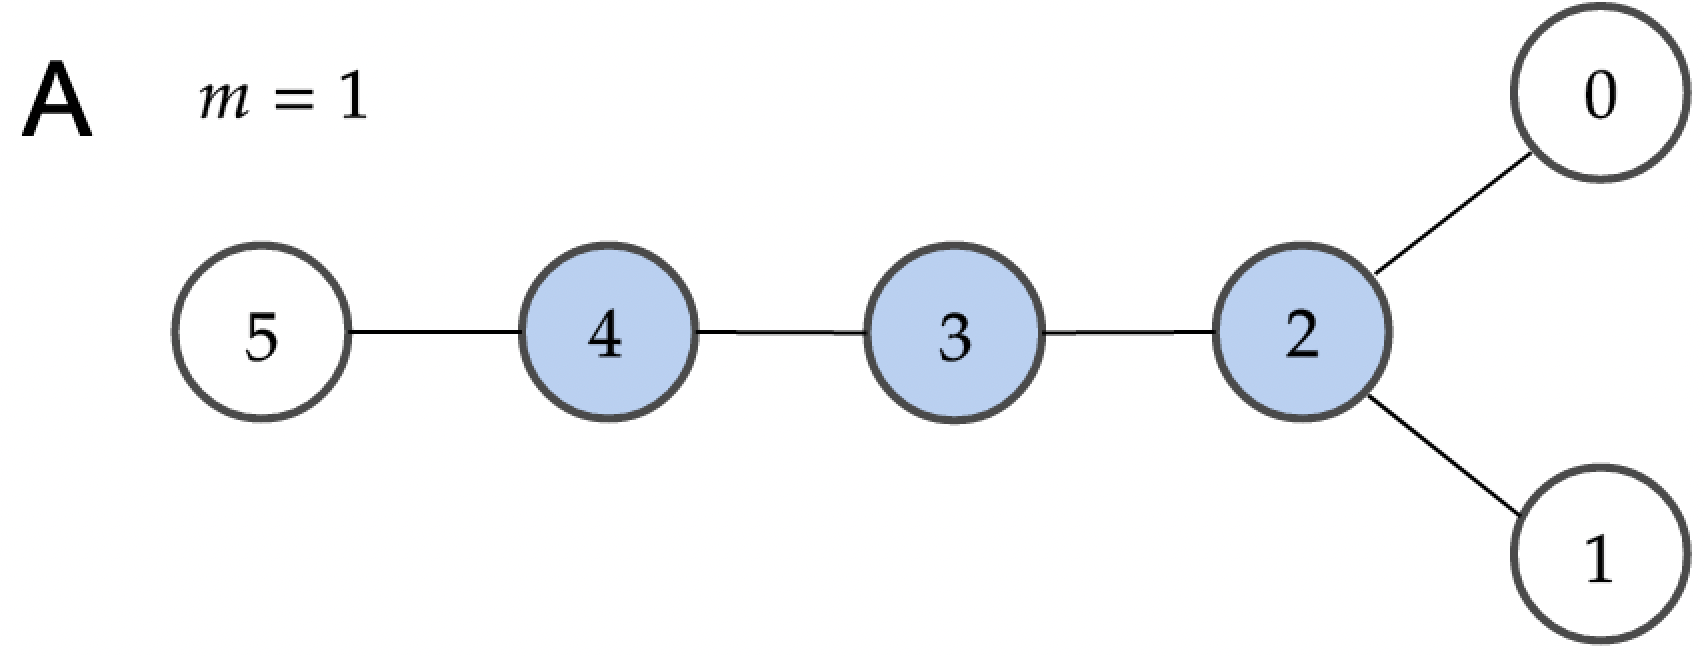
\includegraphics[width=8cm]{latex/Images/input_graph_G_6_0_alternative1.png}
%    \caption{Example input graph. For $m=1$ the algorithm still selects 3 nodes as it is an approximation of the MDS.}
%    \label{fig:input_graph}
%\end{figure}
\begin{rudifig}{\hsize}{Fig. 1: Input Graph}
    
    \hspace{-1em}
    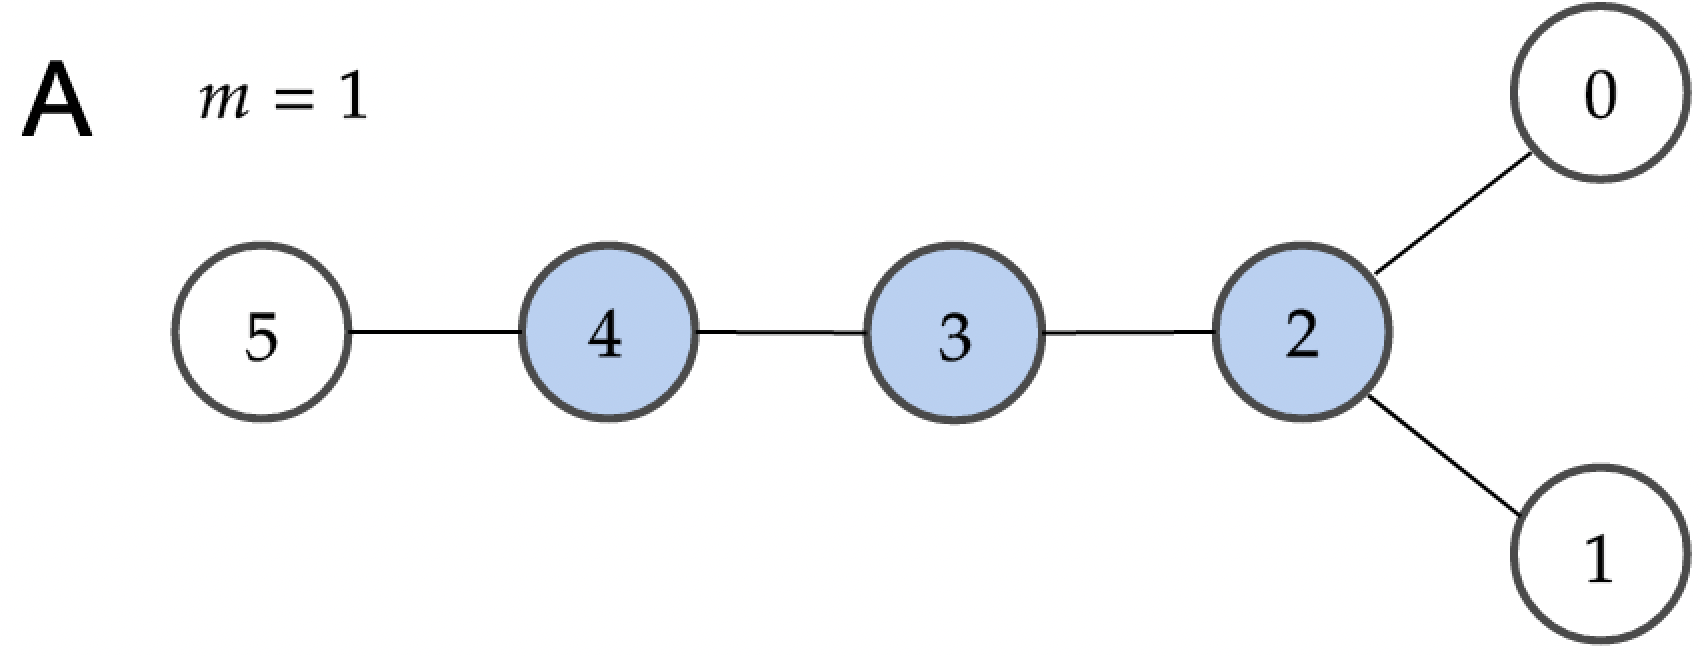
\includegraphics[width=8cm]{latex/Images/input_graph_G_6_0_alternative1.png}
    %\caption{Example input graph. For $m=1$ the algorithm still selects 3 nodes as it is an approximation of the MDS.}
    \label{fig:input_graph}
\end{rudifig}

%\begin{figure}[]
%    \centering
%    %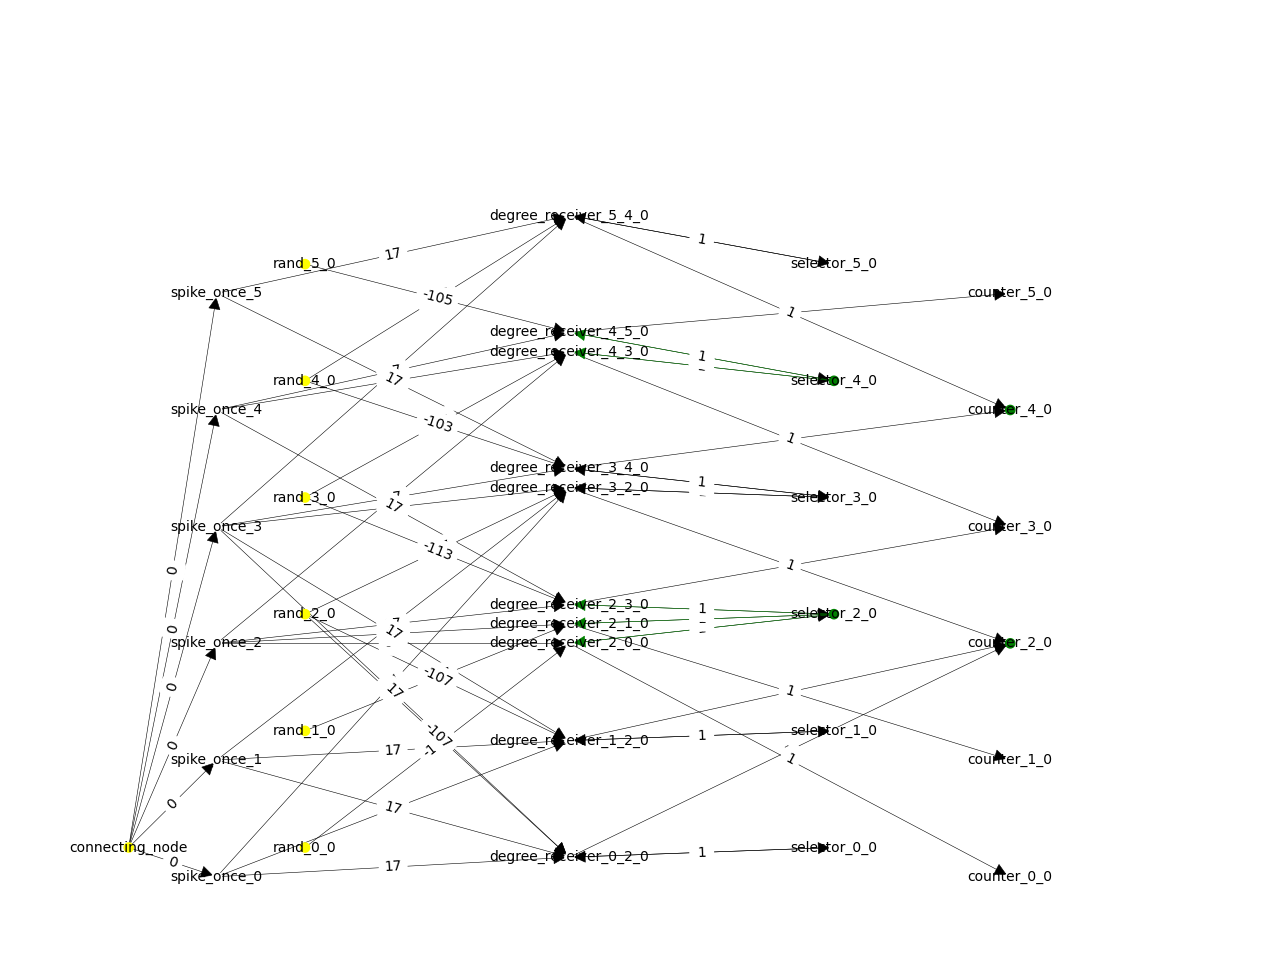
\includegraphics[width=8cm]{latex/Images/structured_graph_snn_m0_n6_iter0_t77.png}
%    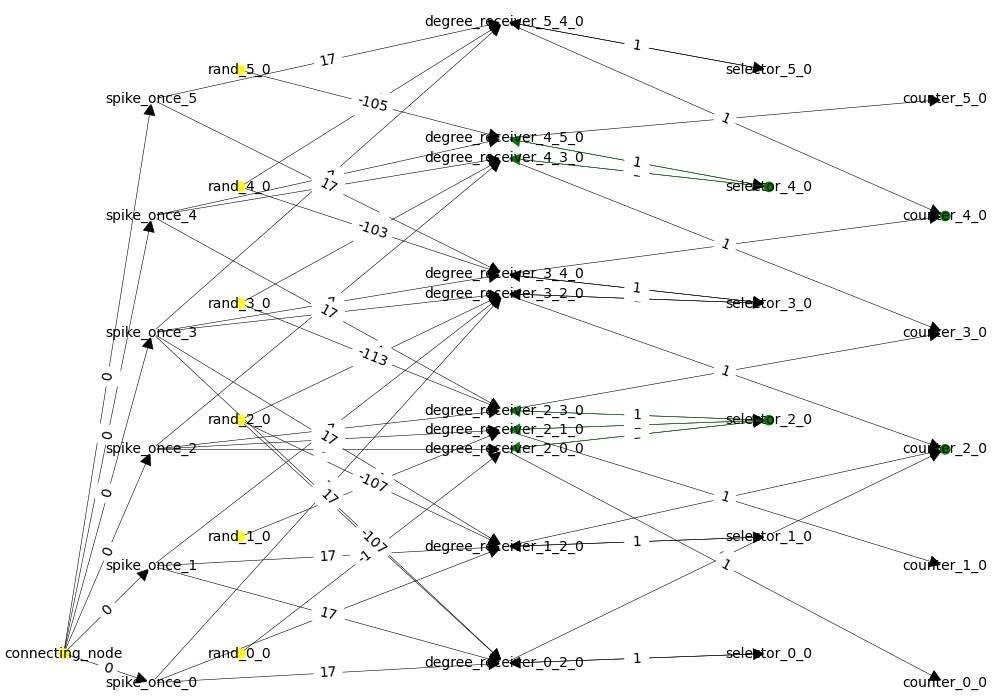
\includegraphics[width=\linewidth]{latex/Images/cropped.jpeg}
%    \caption{Example SNN encoding of algorithm to approximate MDS on the input graph of \cref{fig:input_graph}. This module is connected in series where the mark counter neuron takes up the role of spike\_once neuron in the next round of the approximation algorithm. For a more detailed description of the SNN implementation the reader is referred to Diehl et al. \cite{diehl}. %TODO: update to match updated input graph.
%    }
%    \label{fig:encoded_snn}
%\end{figure}
\begin{rudifig}{\hsize}{Fig. 2: Example SNN}
    
    \hspace{-1em}
    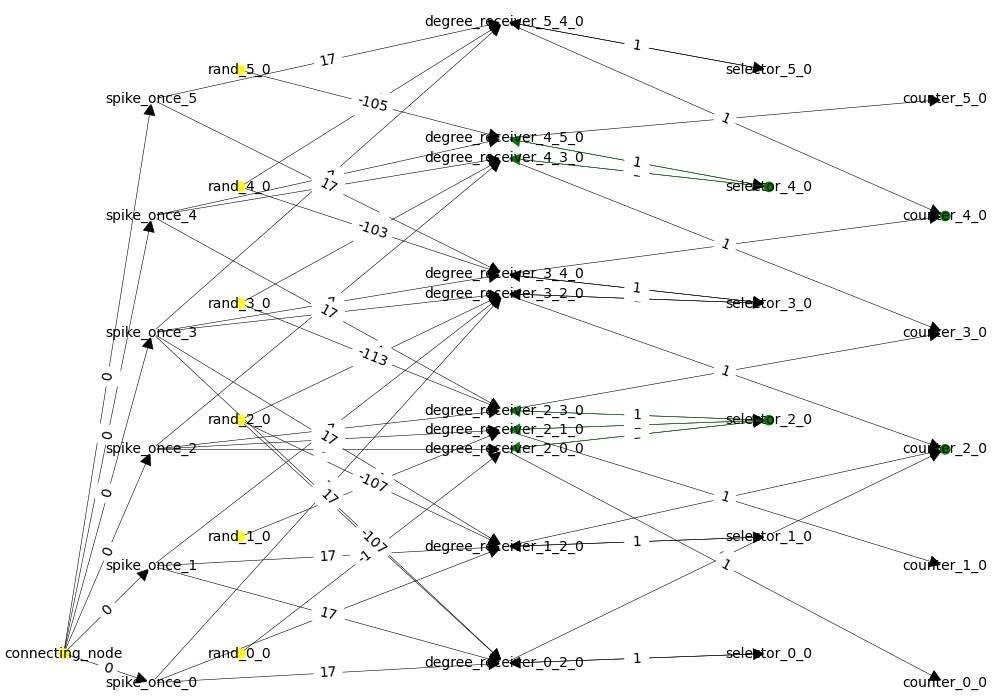
\includegraphics[width=\linewidth]{latex/Images/cropped.jpeg}
    %\caption{Example SNN encoding of algorithm to approximate MDS on the input graph of \cref{fig:input_graph}. This module is connected in series where the mark counter neuron takes up the role of spike\_once neuron in the next round of the approximation algorithm. For a more detailed description of the SNN implementation the reader is referred to Diehl et al. \cite{diehl}. %TODO: update to match updated input graph.
    %}
    \label{fig:encoded_snn}
\end{rudifig}

\noindent This SSN implementation of the MDS approximation algorithm is onwards referred to as the default network. This default network is enhanced with strategically placed redundant neurons that are inhibited by the default network neurons. Next, space radiation damage is simulated on the Loihi 2 in the form of random neuron deaths. These neuron deaths imply that a neuron is removed from the SNN, which can occur in both the default network and the set of redundancy neurons. If a default network neuron dies, the inhibition to the redundant neuron should be removed, causing the SNN to use the alternative neural pathway to recover from this damage. This usage of the alternative neural pathway simulates the multi-pathway structures found in brains of higher vertebrates and is proposed as the main adaptive mechanism in response to damage.

\subsection{Hardware}\label{subsec:hardware}
At the time of writing, no single-event effect (SEEs) propagation mechanisms are identified for space radiation exposure on the Loihi 1 \& 2  neuromorphic chips, a high-level software simulation of these single-event effects is performed. This is done by assuming that the non-neuromorphic components of the chips are performing nominally, and that the SEEs propagate from, for example, transient bit-flips, towards neuronal and synaptic parameter changes. The first assumptions may be accurate if local radiation hardening and redundancy is applied to the non-neuromorphic components. Weight and/or energy saving could be a motivation to apply these radiation counter-measures sparsely. The second assumption is based on the digital nature of the components that make up the neural components of the Loihi. %The components that make up the neural compartments and synapses of the Loihi are visualised in \cref{fig:loihi_micro_architecture}.
%\begin{figure}[H]
%    \centering
%    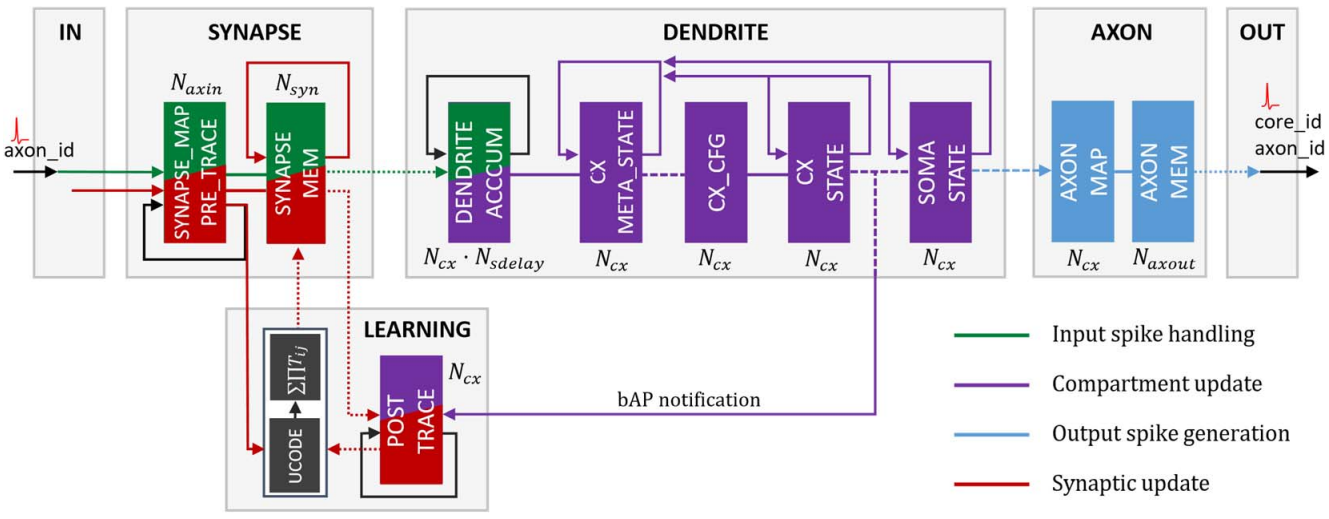
\includegraphics[width=8cm]{latex/Images/loihi_micro_architecture.png}
%    \caption{Core Top-Level Microarchitecture of the Loihi chip. The SYNAPSE unit processes all incoming spikes and
%    reads out the associated synaptic weights from the SRAM memory \cite{davies_loihi_2018}
%    .}
%    \label{fig:loihi_micro_architecture}
%\end{figure}




\subsection{Testing}\label{subsec:testing}
To test whether the brain adaptation implementation may be used to increase radiation robustness of neuromorphic space hardware, it is compared to a baseline without brain adaptation. 

% TODO: verify subsubsections are allowed.
\subsubsection{Metrics}\label{subsubsec:metrics}
The metrics of the comparison are:
\begin{enumerate}
    \item \textit{Radiation Robustness} - a percentage score indicating the ratio of successful solution generation on random input graphs.
    \item \textit{Neuronal \& Synaptic Overcapacity} - a factor from 0 to $n$, indicating the ratio of redundant neurons and synapses with respect to the original implementation without adaptation implementation. % TODO: consistent default network naming see method/intro.
    \item \textit{Energy Efficiency} - the number of spikes consumed by implementations.
    %\item \textit{Time complexity} - the theoretical time complexity required for network initialisation and adaptation.
    %\item \textit{Space Complexity} - the theoretical space complexity required for network initialisation and adaptation.
\end{enumerate}

\subsubsection{Simulated Radiation Damage}\label{subsubsec:simulated_radiation_damage}
This work simulates radiation damage propagation of SEEs as neuron deaths by setting the neuron thresholds $vth=1000 [V]$ at from the start of the simulation. The 1000 [V] is arbitrary yet large enough to prevent spiking. Transient effects are ignored along with neuron property changes in $\delta u,\delta v, bias$, synaptic death, and synaptic property changes in: $sign,weight$.

\subsubsection{Brain Adaptation Mechanism}\label{subsubsec:brain_adaptation_mechanisms}
The selected SNN implementation is enhanced with redundant neurons and neuronal pathways to realise simulated radiation robustness. A basic example is shown in \cref{fig:eg_brain_adaptation}.
% Non poster image:
%\begin{figure}[H]
%    \centering
%    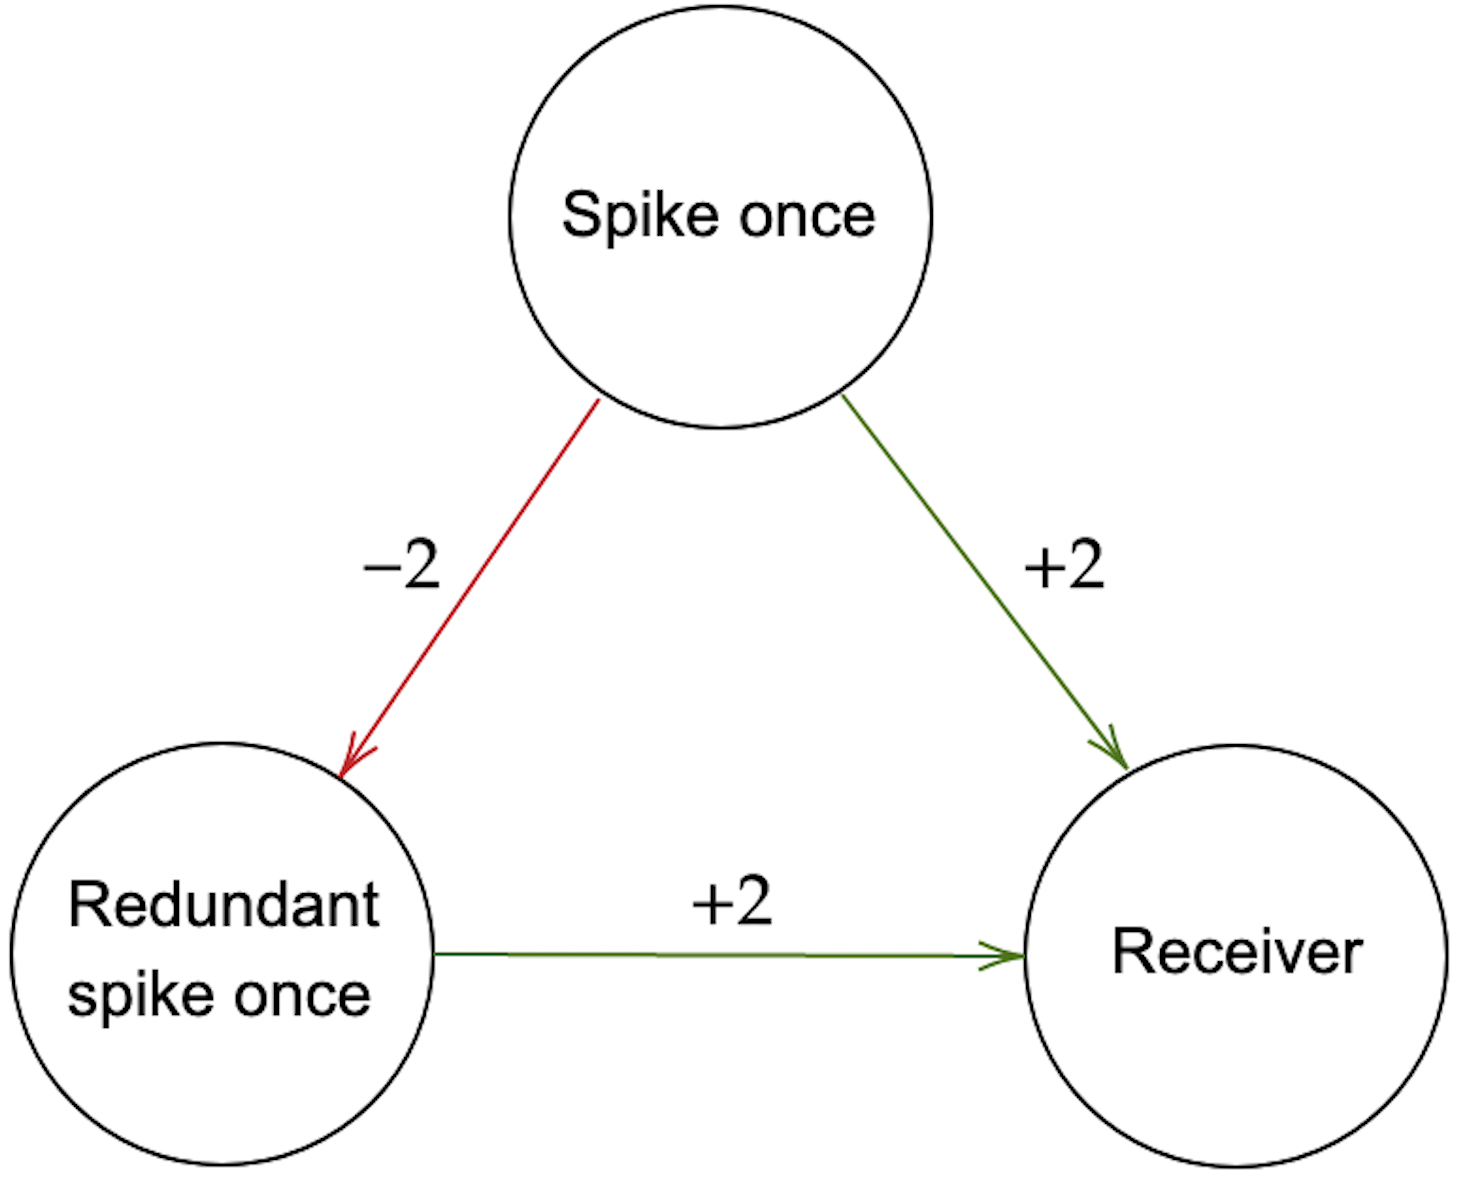
\includegraphics[width=.5\linewidth]{latex/Images/brain_adaptation_alternative.png}
%    \caption{Alternative neural pathway for a redundancy of the spike\_once neuron. If the spike\_once neuron dies due to simulated radiation-induced SEEs ($vth=inf$), the redundancy neuron inhibition is eliminated. Without inhibition, the redundant spike\_once neuron copies the spike\_once behaviour with a delay of 1 timestep.}
%    \label{fig:eg_brain_adaptation}
%\end{figure}
\begin{rudifig}{\hsize}{Fig. 3: Redundancy}
    %
\includegraphics[width=\hsize]{ru_en_1}
    \hspace{-1em}
    %
\includegraphics[width=700pt]{latex/Images/os0.jpg}
    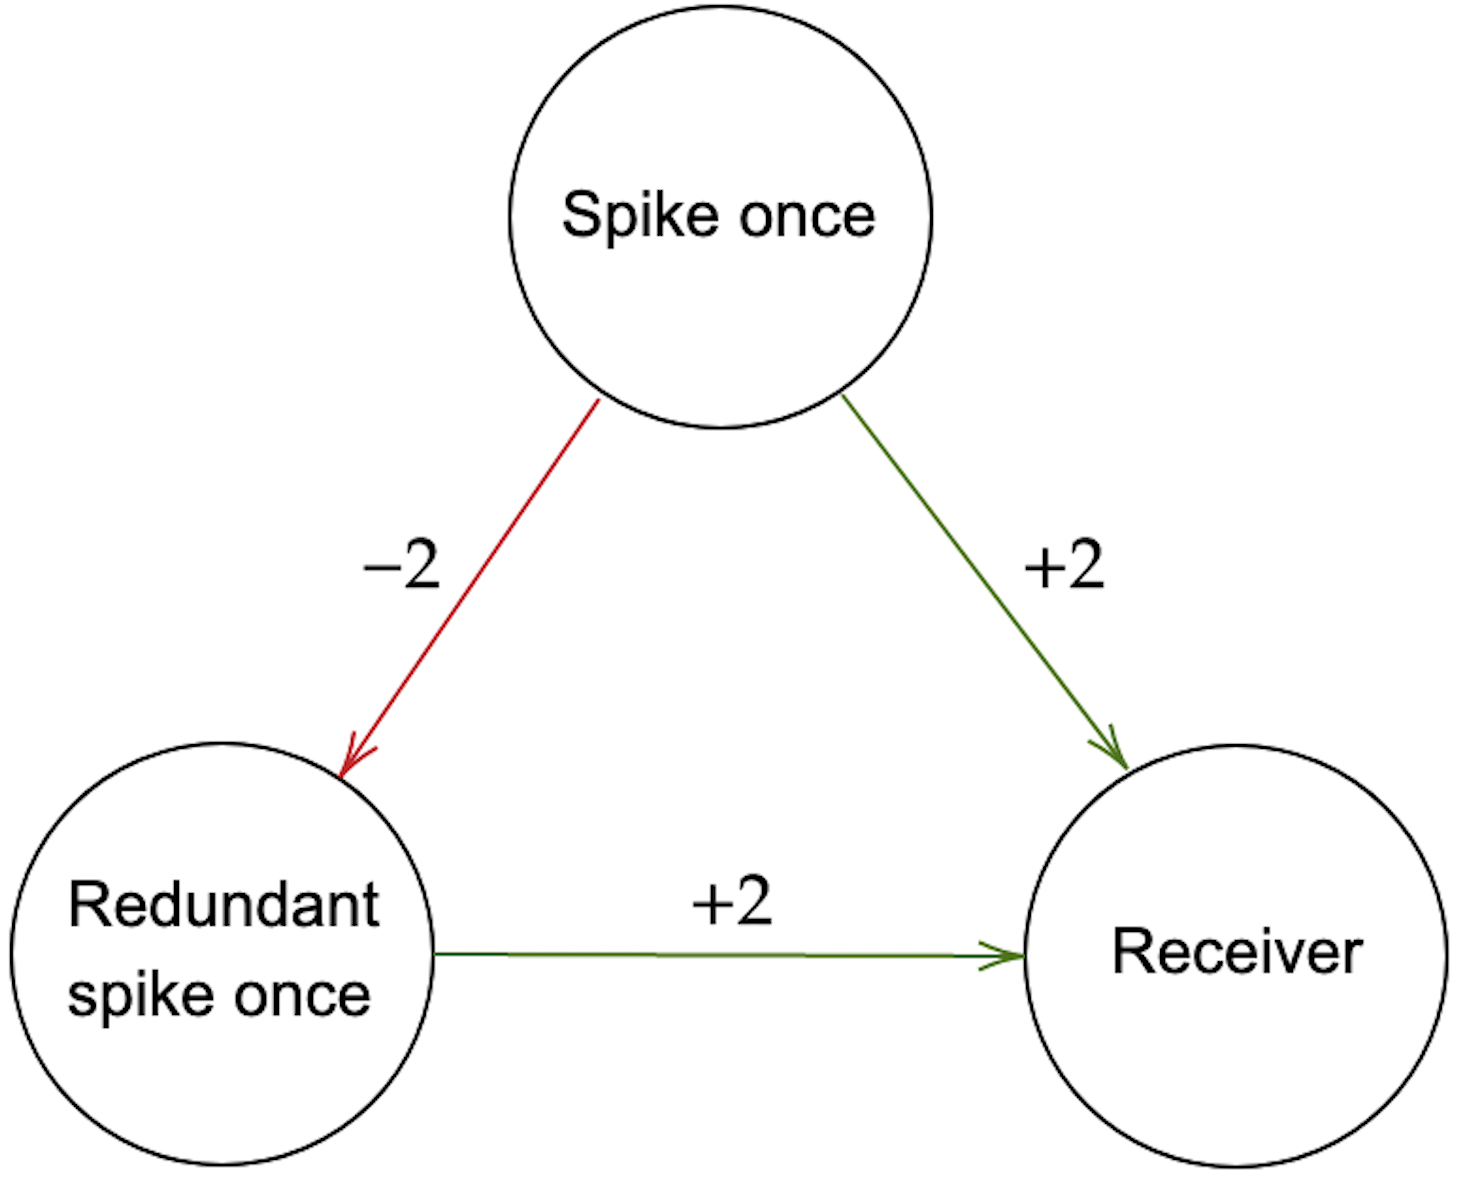
\includegraphics[width=700pt]{latex/Images/brain_adaptation_alternative.png}
    %\caption{Alternative neural pathway for a redundancy of the spike\_once neuron. If the spike\_once neuron dies due to simulated radiation-induced SEEs ($vth=inf$), the redundancy neuron inhibition is eliminated. Without inhibition, the redundant spike\_once neuron copies the spike\_once behaviour with a delay of 1 timestep.}
    \label{fig:eg_brain_adaptation}
\end{rudifig}


\noindent The alternative neural pathway renders a single neuron $original_i$ with $a$ input synapses, and $b$ output synapses, redundant at the cost of $2a+2b$ synapses and 2 neurons. This cost can be reduced by implementing a controller that scans the network and manually redirects neural pathways to a smaller buffer network. However, that shifts the radiation robustness problem as that controller may also endure SEEs. % This does allow local shielding to be used, and may use components that are physically more robust than the SNN networks.
One can also add triple/$n$-factor redundancy by including more redundant spike\_once neurons that are inhibited by the original spike\_once neuron and each other. This induces an additional delay of t=1 time step per redundant neuron.

%\item \textcolor{red}{An Neumann monitoring module that scans the entire SNN network probing its behaviour, and re-routing broken neurons and/or synapses to redundant neurons.}
%\item \textcolor{red}{A rate-coding frequency adaptation to reduce the relative impact of radiation induced spike omission in a subnetwork of the complete SNN implementation of the MDS approximation.}
